\chapter{Result}
The examination based on a machine equipped with Intel(R) Core(TM) i7-4790 CPU 3.6GHz, 16 GB of RAM. For each dataset, it includes 293 images(3264 x 2448). 
The landmarks estimated automatically based on two method: \textit{cross-corrlelation} (called method 1) and \textit{the proposed method} (called method 2). And the result obtained from the method 2 is better than the result from the method 1.
\begin{figure}[h!]
\centering
\subfloat[The scene image]{\label{fig:pht_1}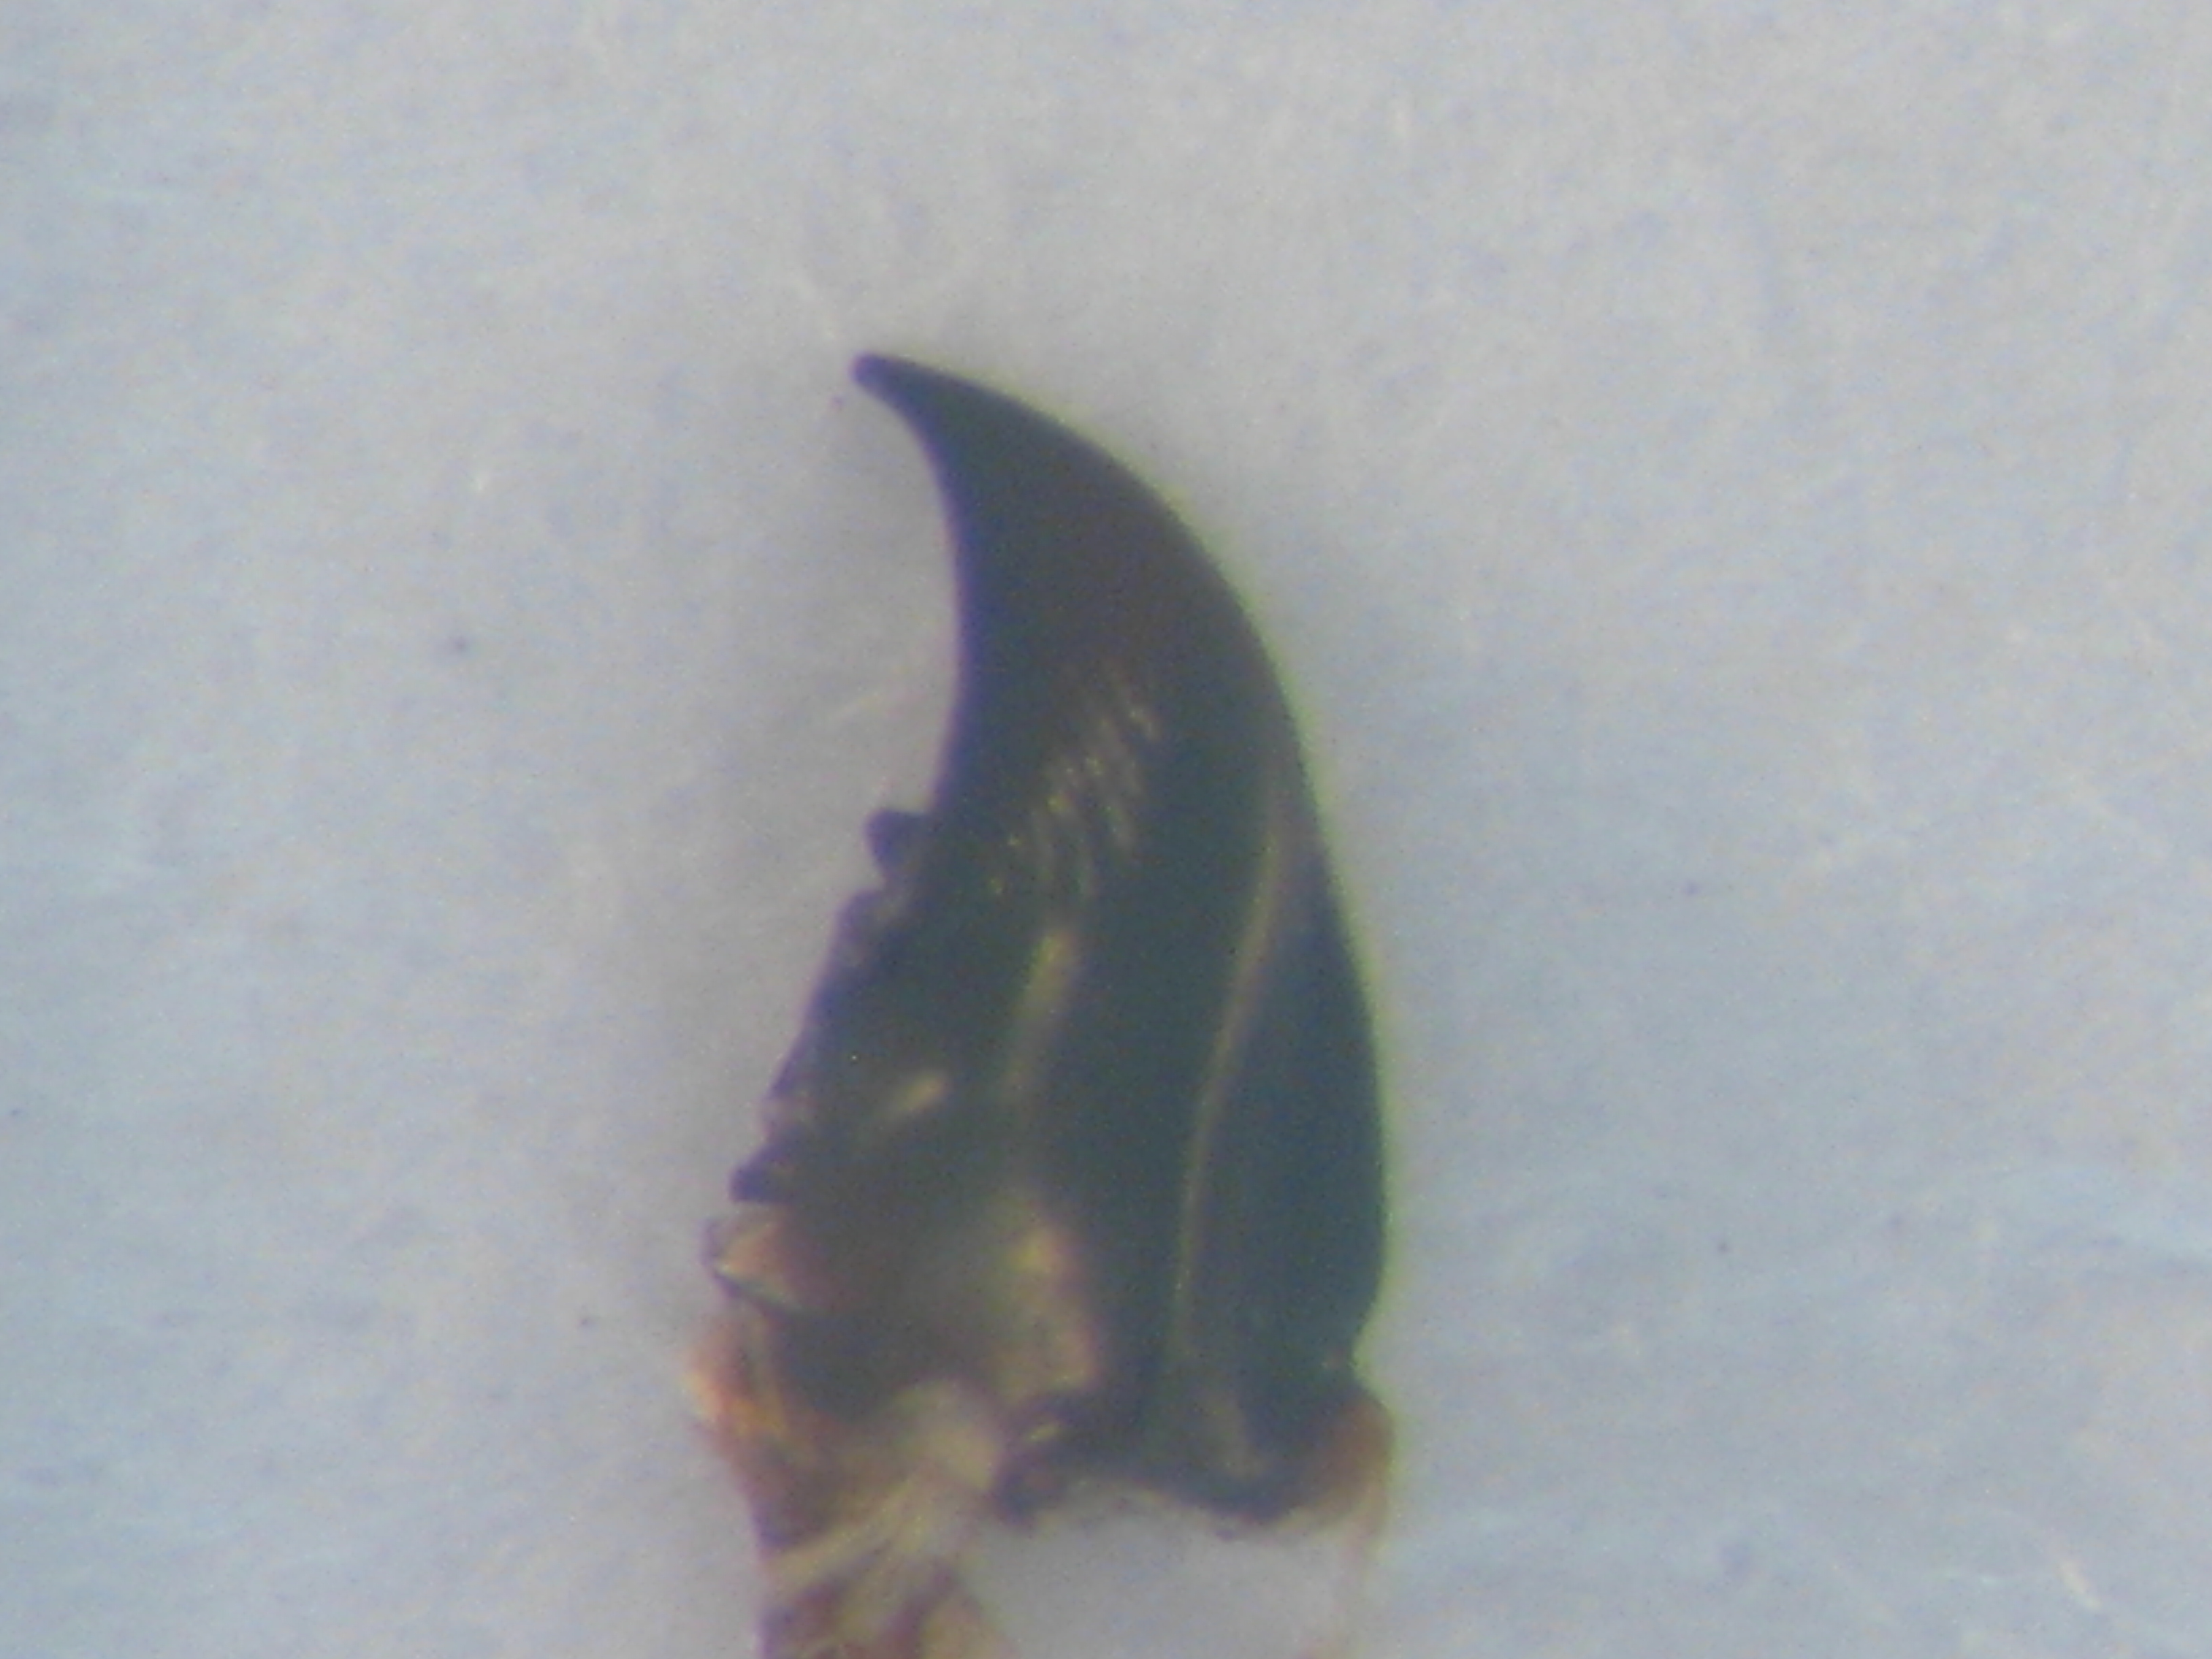
\includegraphics[width=0.45\textwidth]{./images/md32}}~~
\subfloat[The scene image with estimated landmarks ]{\label{fig:pht_2}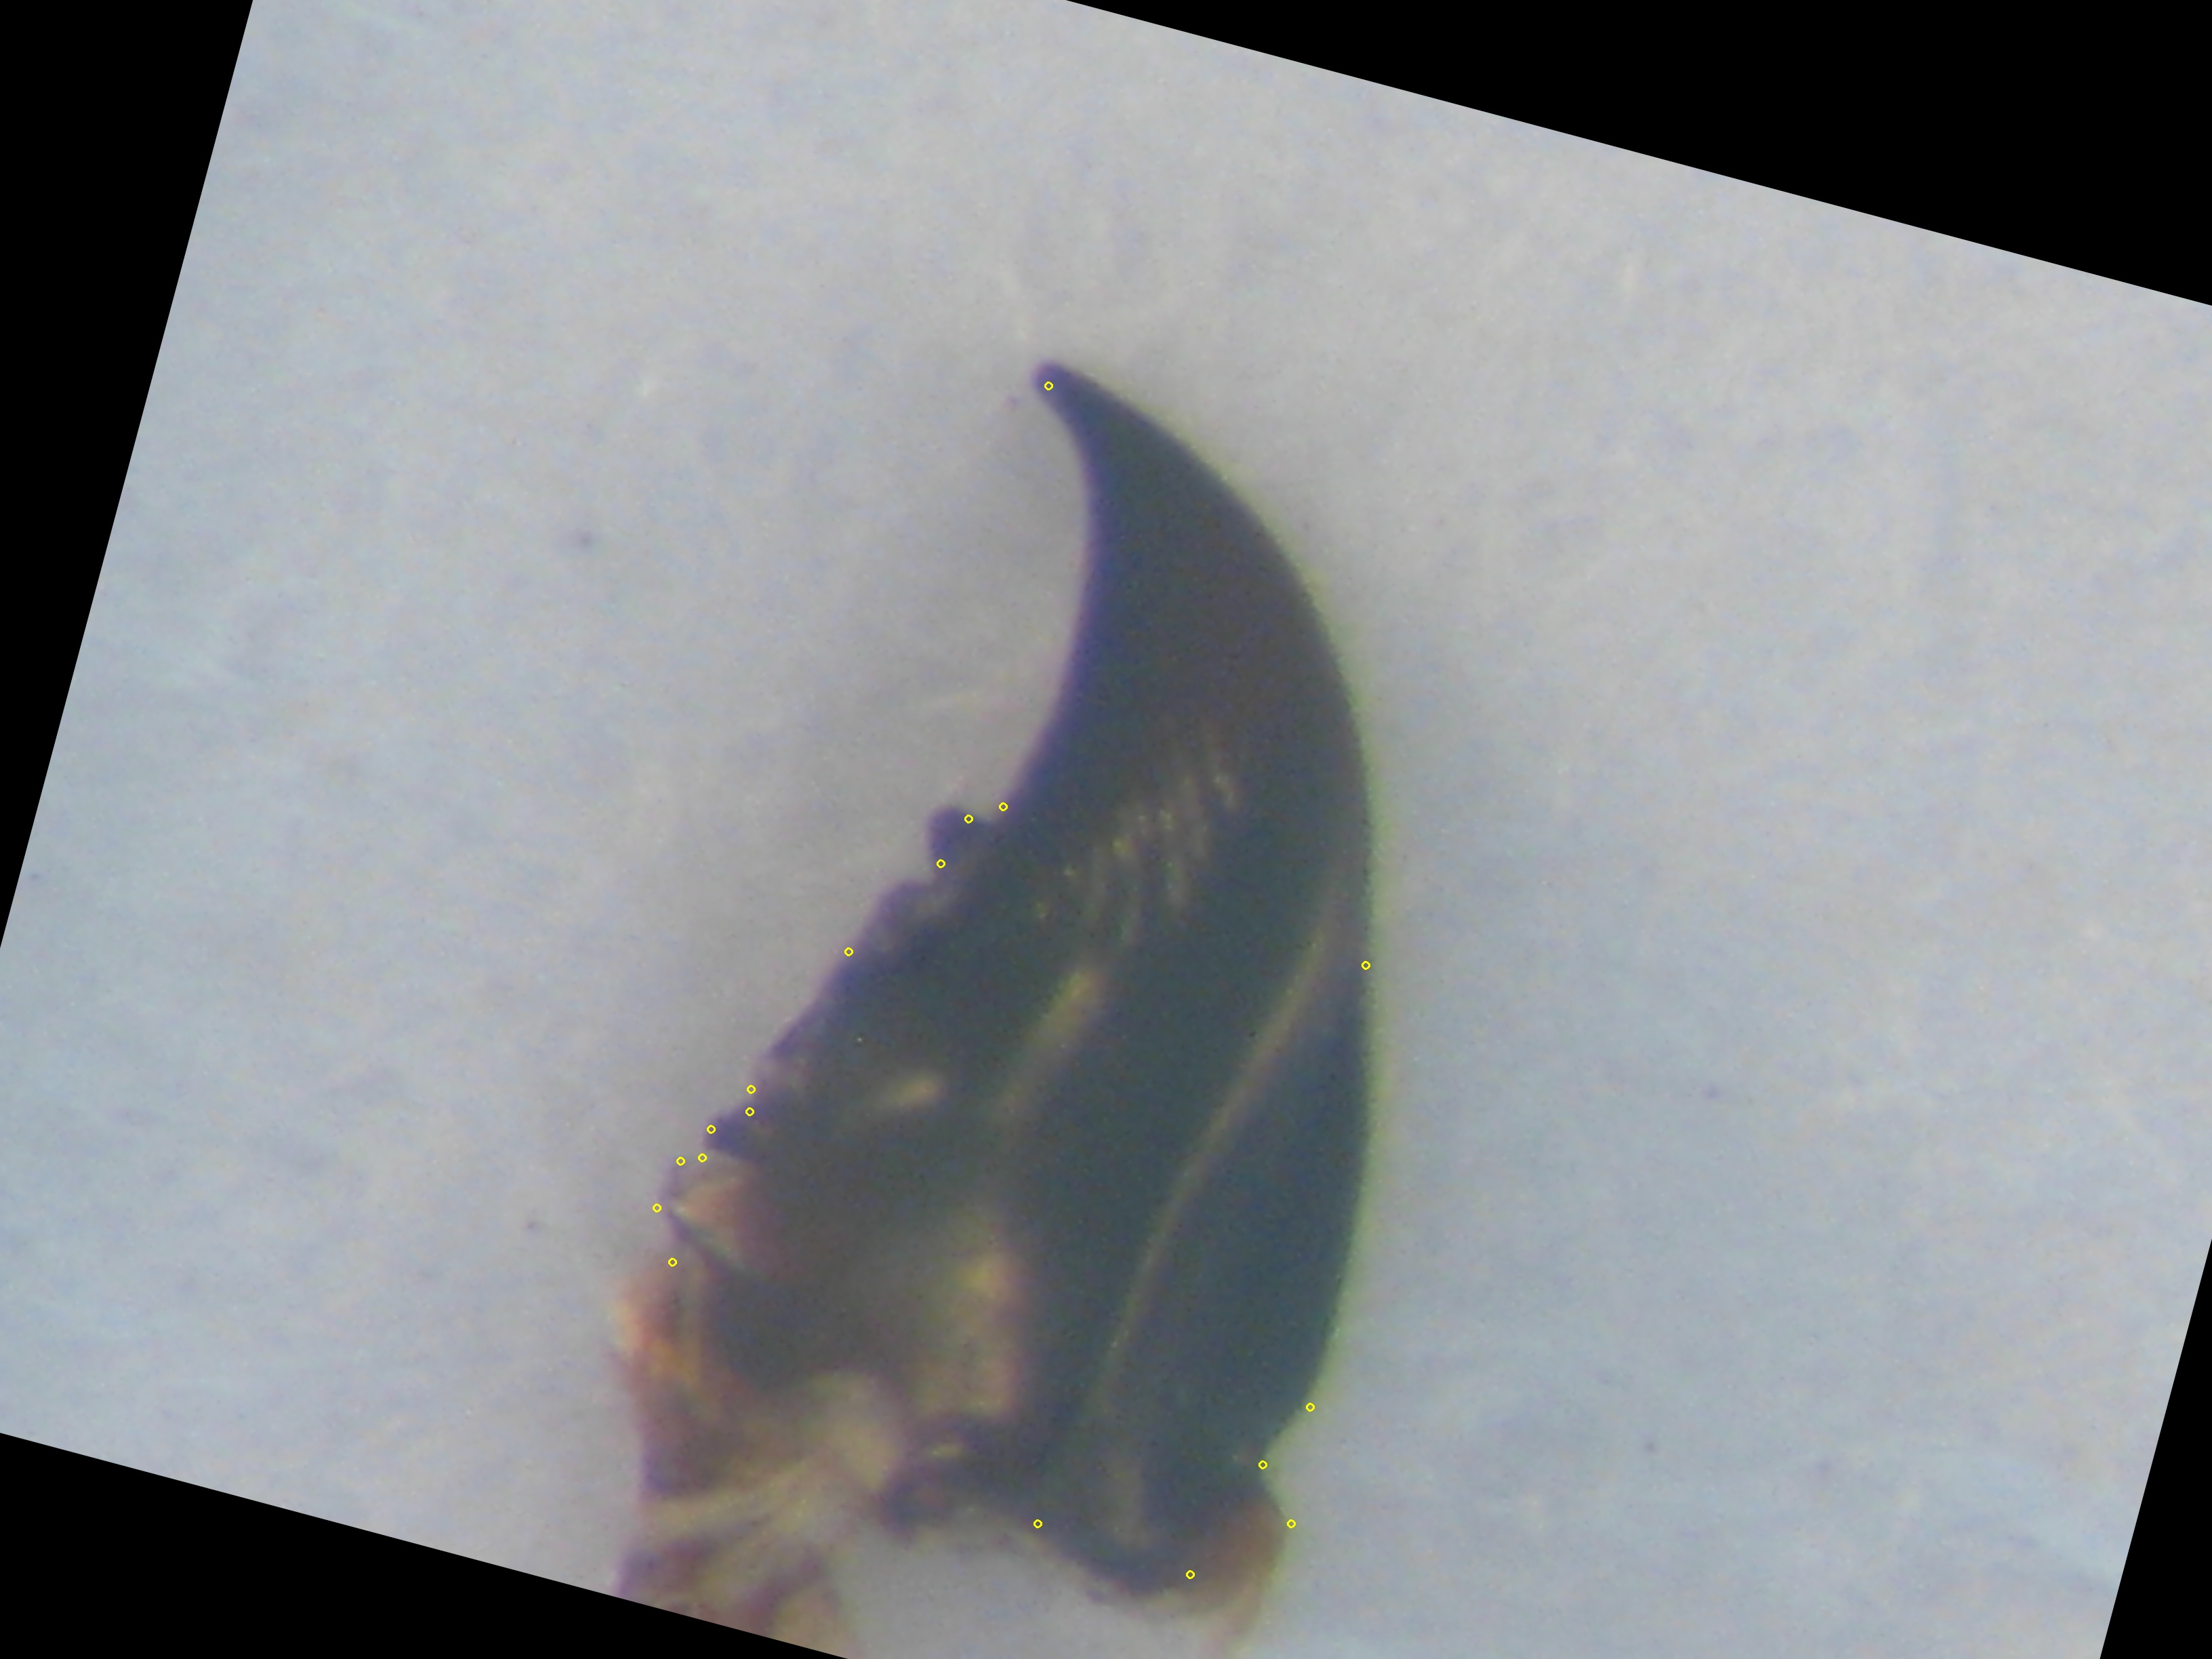
\includegraphics[width=0.45\textwidth]{./images/est32}}
\caption{Automatic identification the landmarks}
\label{fig:figure_31}
\end{figure}